% trilemma.tex — The Attribution Impossibility trilemma figure
% Compiles standalone:  cd paper/figures && pdflatex trilemma.tex
% Include in paper:     
\includegraphics[width=\textwidth]{figures/trilemma.pdf}
%
\documentclass[border=8pt]{standalone}

\usepackage{tikz}
\usepackage{amsmath,amssymb}
\usepackage{xcolor}

\usetikzlibrary{positioning, arrows.meta, calc, decorations.pathreplacing}

\definecolor{familyA}{RGB}{230,120,30}   % orange
\definecolor{familyB}{RGB}{40,100,200}   % blue
\definecolor{impossiblered}{RGB}{200,30,30}
\definecolor{bardark}{RGB}{60,60,60}
\definecolor{barlight}{RGB}{160,160,160}
\definecolor{dashgreen}{RGB}{50,150,80}
\definecolor{trivia}{RGB}{140,140,140}

\begin{document}
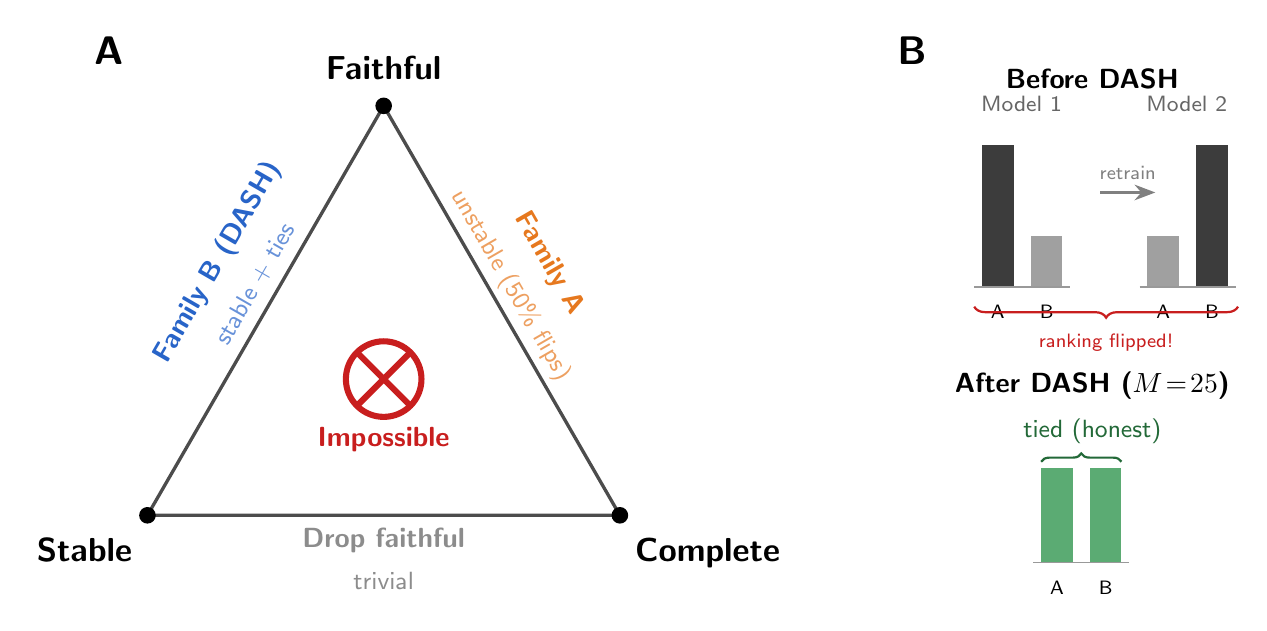
\begin{tikzpicture}[
    every node/.style={font=\sffamily},
    >=Stealth
  ]

  % ============================================================
  %  PANEL A — Trilemma Triangle
  % ============================================================
  \begin{scope}[shift={(0,0)}]

    % Equilateral triangle, side length 6
    \coordinate (F) at (0, 5.2);       % top: Faithful
    \coordinate (S) at (-3.0, 0);      % bottom-left: Stable
    \coordinate (C) at (3.0, 0);       % bottom-right: Complete

    % Draw edges (thick)
    \draw[line width=1.2pt, black!70] (F) -- (S) -- (C) -- cycle;

    % Vertex labels (bold, large)
    \node[above=6pt of F, font=\sffamily\bfseries\large] {Faithful};
    \node[below left=5pt and 2pt of S, font=\sffamily\bfseries\large] {Stable};
    \node[below right=5pt and 2pt of C, font=\sffamily\bfseries\large] {Complete};

    % Small filled circles at vertices
    \fill (F) circle (3pt);
    \fill (S) circle (3pt);
    \fill (C) circle (3pt);

    % --- Central "Impossible" marker (lowered to avoid overlap) ---
    \coordinate (center) at (0, 1.73);

    % Red circle with X (slightly smaller)
    \draw[impossiblered, line width=2.2pt] (center) circle (0.48);
    \draw[impossiblered, line width=2.2pt]
      ($(center)+(-0.33,-0.33)$) -- ($(center)+(0.33,0.33)$);
    \draw[impossiblered, line width=2.2pt]
      ($(center)+(-0.33,0.33)$) -- ($(center)+(0.33,-0.33)$);

    % "Impossible" text (more space below the X)
    \node[below=14pt of center, font=\sffamily\bfseries,
          text=impossiblered] {Impossible};

    % --- Edge annotations (pulled away from edges) ---

    % Left edge: Family B (DASH) — main label (outside triangle)
    \node[rotate=60, anchor=south, font=\sffamily\bfseries,
          text=familyB] at ($(F)!0.45!(S) + (-0.5,0.2)$)
      {Family B (DASH)};
    % Subtitle below main label (further from edge = more negative perpendicular)
    \node[rotate=60, anchor=north, font=\sffamily\small,
          text=familyB!70] at ($(F)!0.45!(S) + (-0.5,0.2)$)
      {stable $+$ ties};

    % Right edge: Family A — main label (outside triangle)
    \node[rotate=-60, anchor=south, font=\sffamily\bfseries,
          text=familyA] at ($(F)!0.45!(C) + (0.5,0.2)$)
      {Family A};
    % Subtitle below main label
    \node[rotate=-60, anchor=north, font=\sffamily\small,
          text=familyA!70] at ($(F)!0.45!(C) + (0.5,0.2)$)
      {unstable (50\% flips)};

    % Bottom edge: Drop faithful
    \node[anchor=south, font=\sffamily\bfseries,
          text=trivia] at ($(S)!0.5!(C) + (0,-0.6)$)
      {Drop faithful};
    \node[anchor=north, font=\sffamily\small,
          text=trivia] at ($(S)!0.5!(C) + (0,-0.6)$)
      {trivial};

    % Panel label
    \node[anchor=north west, font=\sffamily\bfseries\Large]
      at (-3.8, 6.2) {\textsf{A}};

  \end{scope}

  % ============================================================
  %  PANEL B — Before / After DASH (right side, wider)
  % ============================================================
  \begin{scope}[shift={(8.0, -0.3)}]

    \newcommand{\barwidth}{0.4}
    \newcommand{\gapwidth}{0.22}

    % Panel label
    \node[anchor=north west, font=\sffamily\bfseries\Large]
      at (-1.6, 6.5) {\textsf{B}};

    % ----------------------------------------------------------
    %  Top sub-panel: Before DASH
    % ----------------------------------------------------------
    \node[anchor=south, font=\sffamily\bfseries]
      at (1.0, 5.6) {Before DASH};

    % Model 1 (left bar chart)
    \begin{scope}[shift={(-0.4, 3.2)}]
      \node[anchor=south, font=\sffamily\footnotesize, text=black!60]
        at (0.5, 2.1) {Model 1};

      % Feature A: tall
      \fill[bardark] (0, 0) rectangle (\barwidth, 1.8);
      \node[below=3pt, font=\sffamily\scriptsize] at (\barwidth/2, 0) {A};

      % Feature B: short
      \fill[barlight] (\barwidth+\gapwidth, 0)
        rectangle (2*\barwidth+\gapwidth, 0.65);
      \node[below=3pt, font=\sffamily\scriptsize]
        at (\barwidth+\gapwidth+\barwidth/2, 0) {B};

      % Baseline
      \draw[black!40] (-0.1, 0) -- (2*\barwidth+\gapwidth+0.1, 0);
    \end{scope}

    % "retrain" arrow (more space between charts)
    \draw[->, line width=1pt, black!50]
      (1.1, 4.4) -- (1.8, 4.4)
      node[midway, above=1pt, font=\sffamily\scriptsize, text=black!50] {retrain};

    % Model 2 (right bar chart) — reversed
    \begin{scope}[shift={(1.7, 3.2)}]
      \node[anchor=south, font=\sffamily\footnotesize, text=black!60]
        at (0.5, 2.1) {Model 2};

      % Feature A: short (flipped!)
      \fill[barlight] (0, 0) rectangle (\barwidth, 0.65);
      \node[below=3pt, font=\sffamily\scriptsize] at (\barwidth/2, 0) {A};

      % Feature B: tall (flipped!)
      \fill[bardark] (\barwidth+\gapwidth, 0)
        rectangle (2*\barwidth+\gapwidth, 1.8);
      \node[below=3pt, font=\sffamily\scriptsize]
        at (\barwidth+\gapwidth+\barwidth/2, 0) {B};

      % Baseline
      \draw[black!40] (-0.1, 0) -- (2*\barwidth+\gapwidth+0.1, 0);
    \end{scope}

    % Red brace annotation: ranking flipped (below baselines with space)
    \draw[impossiblered, thick, decorate,
          decoration={brace, amplitude=4pt, mirror}]
      (-0.5, 2.95) -- (2.85, 2.95)
      node[midway, below=6pt, font=\sffamily\scriptsize,
           text=impossiblered] {ranking flipped!};

    % ----------------------------------------------------------
    %  Bottom sub-panel: After DASH (M=25) — generous spacing
    % ----------------------------------------------------------
    \node[anchor=south, font=\sffamily\bfseries]
      at (1.0, 1.65) {After DASH ($M\!=\!25$)};

    % "tied (honest)" label below the title
    \node[anchor=north, font=\sffamily\small,
          text=dashgreen!70!black]
      at (1.0, 1.65) {tied (honest)};

    % Single bar chart — tied
    \begin{scope}[shift={(0.35, -0.3)}]
      % Feature A
      \fill[dashgreen!80] (0, 0) rectangle (\barwidth, 1.2);
      \node[below=3pt, font=\sffamily\scriptsize] at (\barwidth/2, 0) {A};

      % Feature B — same height (tied)
      \fill[dashgreen!80] (\barwidth+\gapwidth, 0)
        rectangle (2*\barwidth+\gapwidth, 1.2);
      \node[below=3pt, font=\sffamily\scriptsize]
        at (\barwidth+\gapwidth+\barwidth/2, 0) {B};

      % Baseline
      \draw[black!40] (-0.1, 0) -- (2*\barwidth+\gapwidth+0.1, 0);

      % Tie bracket above bars
      \draw[dashgreen!70!black, thick, decorate,
            decoration={brace, amplitude=3pt}]
        (0, 1.28) -- (2*\barwidth+\gapwidth, 1.28);
    \end{scope}

  \end{scope}

\end{tikzpicture}
\end{document}
